\documentclass[]{article}
\usepackage{lmodern}
\usepackage{amssymb,amsmath}
\usepackage{ifxetex,ifluatex}
\usepackage{fixltx2e} % provides \textsubscript
\ifnum 0\ifxetex 1\fi\ifluatex 1\fi=0 % if pdftex
  \usepackage[T1]{fontenc}
  \usepackage[utf8]{inputenc}
\else % if luatex or xelatex
  \ifxetex
    \usepackage{mathspec}
    \usepackage{xltxtra,xunicode}
  \else
    \usepackage{fontspec}
  \fi
  \defaultfontfeatures{Mapping=tex-text,Scale=MatchLowercase}
  \newcommand{\euro}{€}
\fi
% use upquote if available, for straight quotes in verbatim environments
\IfFileExists{upquote.sty}{\usepackage{upquote}}{}
% use microtype if available
\IfFileExists{microtype.sty}{%
\usepackage{microtype}
\UseMicrotypeSet[protrusion]{basicmath} % disable protrusion for tt fonts
}{}
\usepackage[margin=1in]{geometry}
\usepackage{color}
\usepackage{fancyvrb}
\newcommand{\VerbBar}{|}
\newcommand{\VERB}{\Verb[commandchars=\\\{\}]}
\DefineVerbatimEnvironment{Highlighting}{Verbatim}{commandchars=\\\{\}}
% Add ',fontsize=\small' for more characters per line
\usepackage{framed}
\definecolor{shadecolor}{RGB}{248,248,248}
\newenvironment{Shaded}{\begin{snugshade}}{\end{snugshade}}
\newcommand{\KeywordTok}[1]{\textcolor[rgb]{0.13,0.29,0.53}{\textbf{{#1}}}}
\newcommand{\DataTypeTok}[1]{\textcolor[rgb]{0.13,0.29,0.53}{{#1}}}
\newcommand{\DecValTok}[1]{\textcolor[rgb]{0.00,0.00,0.81}{{#1}}}
\newcommand{\BaseNTok}[1]{\textcolor[rgb]{0.00,0.00,0.81}{{#1}}}
\newcommand{\FloatTok}[1]{\textcolor[rgb]{0.00,0.00,0.81}{{#1}}}
\newcommand{\CharTok}[1]{\textcolor[rgb]{0.31,0.60,0.02}{{#1}}}
\newcommand{\StringTok}[1]{\textcolor[rgb]{0.31,0.60,0.02}{{#1}}}
\newcommand{\CommentTok}[1]{\textcolor[rgb]{0.56,0.35,0.01}{\textit{{#1}}}}
\newcommand{\OtherTok}[1]{\textcolor[rgb]{0.56,0.35,0.01}{{#1}}}
\newcommand{\AlertTok}[1]{\textcolor[rgb]{0.94,0.16,0.16}{{#1}}}
\newcommand{\FunctionTok}[1]{\textcolor[rgb]{0.00,0.00,0.00}{{#1}}}
\newcommand{\RegionMarkerTok}[1]{{#1}}
\newcommand{\ErrorTok}[1]{\textbf{{#1}}}
\newcommand{\NormalTok}[1]{{#1}}
\usepackage{longtable,booktabs}
\usepackage{graphicx}
\makeatletter
\def\maxwidth{\ifdim\Gin@nat@width>\linewidth\linewidth\else\Gin@nat@width\fi}
\def\maxheight{\ifdim\Gin@nat@height>\textheight\textheight\else\Gin@nat@height\fi}
\makeatother
% Scale images if necessary, so that they will not overflow the page
% margins by default, and it is still possible to overwrite the defaults
% using explicit options in \includegraphics[width, height, ...]{}
\setkeys{Gin}{width=\maxwidth,height=\maxheight,keepaspectratio}
\ifxetex
  \usepackage[setpagesize=false, % page size defined by xetex
              unicode=false, % unicode breaks when used with xetex
              xetex]{hyperref}
\else
  \usepackage[unicode=true]{hyperref}
\fi
\hypersetup{breaklinks=true,
            bookmarks=true,
            pdfauthor={Siyuan Meng},
            pdftitle={Impact of HbA1c Measurement on Hospital Readmission Rates},
            colorlinks=true,
            citecolor=blue,
            urlcolor=blue,
            linkcolor=magenta,
            pdfborder={0 0 0}}
\urlstyle{same}  % don't use monospace font for urls
\setlength{\parindent}{0pt}
\setlength{\parskip}{6pt plus 2pt minus 1pt}
\setlength{\emergencystretch}{3em}  % prevent overfull lines
\setcounter{secnumdepth}{0}

%%% Use protect on footnotes to avoid problems with footnotes in titles
\let\rmarkdownfootnote\footnote%
\def\footnote{\protect\rmarkdownfootnote}

%%% Change title format to be more compact
\usepackage{titling}

% Create subtitle command for use in maketitle
\newcommand{\subtitle}[1]{
  \posttitle{
    \begin{center}\large#1\end{center}
    }
}

\setlength{\droptitle}{-2em}
  \title{Impact of HbA1c Measurement on Hospital Readmission Rates}
  \pretitle{\vspace{\droptitle}\centering\huge}
  \posttitle{\par}
  \author{Siyuan Meng}
  \preauthor{\centering\large\emph}
  \postauthor{\par}
  \predate{\centering\large\emph}
  \postdate{\par}
  \date{December 4, 2015}



\begin{document}

\maketitle


\section{Reproducibility}\label{reproducibility}

In order to get the same results, need certain set of packages, as well
as setting a pseudo-random seed equal the one I used.

\begin{itemize}
\itemsep1pt\parskip0pt\parsep0pt
\item
  The following libraries were used for this project:
\end{itemize}

\begin{Shaded}
\begin{Highlighting}[]
\KeywordTok{library}\NormalTok{(caret)}
\end{Highlighting}
\end{Shaded}

\begin{verbatim}
## Loading required package: lattice
## Loading required package: ggplot2
\end{verbatim}

\begin{Shaded}
\begin{Highlighting}[]
\KeywordTok{library}\NormalTok{(randomForest)}
\end{Highlighting}
\end{Shaded}

\begin{verbatim}
## randomForest 4.6-12
## Type rfNews() to see new features/changes/bug fixes.
\end{verbatim}

\begin{Shaded}
\begin{Highlighting}[]
\KeywordTok{library}\NormalTok{(pander)}
\end{Highlighting}
\end{Shaded}

\begin{itemize}
\itemsep1pt\parskip0pt\parsep0pt
\item
  Here is the seed I set to generate pseudo-random numbers for spliting
  training and test dataset. (see \texttt{Preprocessing} section)
\end{itemize}

\begin{Shaded}
\begin{Highlighting}[]
\KeywordTok{set.seed}\NormalTok{(}\DecValTok{12345}\NormalTok{)}
\end{Highlighting}
\end{Shaded}

\section{Getting data}\label{getting-data}

\begin{Shaded}
\begin{Highlighting}[]
\KeywordTok{setwd}\NormalTok{(}\StringTok{"~/Documents/2015Fall/EE660/EE660_Project"}\NormalTok{)}
\NormalTok{data <-}\StringTok{ }\KeywordTok{read.csv}\NormalTok{(}\StringTok{"~/Documents/2015Fall/EE660/Project/diabetic_data.csv"}\NormalTok{,}
                 \DataTypeTok{stringsAsFactors=}\NormalTok{T,}\DataTypeTok{na.strings =} \StringTok{'?'}\NormalTok{)}
\KeywordTok{dim}\NormalTok{(data)}
\end{Highlighting}
\end{Shaded}

\begin{verbatim}
## [1] 101766     50
\end{verbatim}

\section{Cleaning data}\label{cleaning-data}

The original missing value information can be found in
\url{http://www.hindawi.com/journals/bmri/2014/781670/tab1/}. For
simplicity, only show features which have missing values. (cite)

\begin{longtable}[c]{@{}cccc@{}}
\toprule
\begin{minipage}[b]{0.20\columnwidth}\centering\strut
Feature\_name
\strut\end{minipage} &
\begin{minipage}[b]{0.09\columnwidth}\centering\strut
Type
\strut\end{minipage} &
\begin{minipage}[b]{0.35\columnwidth}\centering\strut
Discription
\strut\end{minipage} &
\begin{minipage}[b]{0.24\columnwidth}\centering\strut
Propotional\_missing
\strut\end{minipage}\tabularnewline
\midrule
\endhead
\begin{minipage}[t]{0.20\columnwidth}\centering\strut
Race
\strut\end{minipage} &
\begin{minipage}[t]{0.09\columnwidth}\centering\strut
Nominal
\strut\end{minipage} &
\begin{minipage}[t]{0.35\columnwidth}\centering\strut
Values: Caucasian, Asian, African American, Hispanic, and other
\strut\end{minipage} &
\begin{minipage}[t]{0.24\columnwidth}\centering\strut
2\%
\strut\end{minipage}\tabularnewline
\begin{minipage}[t]{0.20\columnwidth}\centering\strut
Weight
\strut\end{minipage} &
\begin{minipage}[t]{0.09\columnwidth}\centering\strut
Numeric
\strut\end{minipage} &
\begin{minipage}[t]{0.35\columnwidth}\centering\strut
Weight in pounds
\strut\end{minipage} &
\begin{minipage}[t]{0.24\columnwidth}\centering\strut
97\%
\strut\end{minipage}\tabularnewline
\begin{minipage}[t]{0.20\columnwidth}\centering\strut
Payer code
\strut\end{minipage} &
\begin{minipage}[t]{0.09\columnwidth}\centering\strut
Nominal
\strut\end{minipage} &
\begin{minipage}[t]{0.35\columnwidth}\centering\strut
Integer identifier corresponding to 23 distinct values, for example,
Blue Cross/Blue Shield, Medicare, and self-pay
\strut\end{minipage} &
\begin{minipage}[t]{0.24\columnwidth}\centering\strut
40\%
\strut\end{minipage}\tabularnewline
\begin{minipage}[t]{0.20\columnwidth}\centering\strut
Medical specialty
\strut\end{minipage} &
\begin{minipage}[t]{0.09\columnwidth}\centering\strut
Nominal
\strut\end{minipage} &
\begin{minipage}[t]{0.35\columnwidth}\centering\strut
Integer identifier of a specialty of the admitting physician,
corresponding to 84 distinct values
\strut\end{minipage} &
\begin{minipage}[t]{0.24\columnwidth}\centering\strut
50\%
\strut\end{minipage}\tabularnewline
\begin{minipage}[t]{0.20\columnwidth}\centering\strut
Diagnosis 3
\strut\end{minipage} &
\begin{minipage}[t]{0.09\columnwidth}\centering\strut
Nominal
\strut\end{minipage} &
\begin{minipage}[t]{0.35\columnwidth}\centering\strut
Additional secondary diagnosis (coded as first three digits of ICD9),
corresponding to 954 distinct values
\strut\end{minipage} &
\begin{minipage}[t]{0.24\columnwidth}\centering\strut
1\%
\strut\end{minipage}\tabularnewline
\bottomrule
\end{longtable}

The way I deal with missing values is to delete \texttt{Weight},
\texttt{Payer code} and \texttt{Medical speciality} feaures (columns),
since all three features have more than 50\% missing values and then
delete samples (rows) which has missing values.

\begin{Shaded}
\begin{Highlighting}[]
\NormalTok{data <-}\StringTok{ }\NormalTok{data[,}\KeywordTok{c}\NormalTok{(-}\DecValTok{6}\NormalTok{,-}\DecValTok{11}\NormalTok{,-}\DecValTok{12}\NormalTok{)]}
\NormalTok{data <-}\StringTok{ }\KeywordTok{na.omit}\NormalTok{(data)}
\KeywordTok{dim}\NormalTok{(data)}
\end{Highlighting}
\end{Shaded}

\begin{verbatim}
## [1] 98053    47
\end{verbatim}

In general, should split the original data into training and testing
first and then deal with the missing values. However, both methods will
yield same dimension \texttt{data}. For simplicity, deal with NAs first
here.

\section{Preprocessing}\label{preprocessing}

(Preprocessing is more crucial when using model based algorithms,
e.g.~Linear Discrimant Analysis, Naive Bayes, Linear
Regression\ldots{}than using non-parametrical algorithms.)

\begin{itemize}
\item
  There are also other ways to impute data, like knnimpute\ldots{}For
  convenience, try omitting NA rows first.
\item
  Kill the first two features(\texttt{encounter\_id} and
  \texttt{patient\_nbr}) which are ids for encounted and patients. They
  are not considered relevant to the outcome. Also, extract label
  column, which is the last column of \texttt{data}.
\end{itemize}

\begin{Shaded}
\begin{Highlighting}[]
\NormalTok{data <-}\StringTok{ }\NormalTok{data[,}\KeywordTok{c}\NormalTok{(-}\DecValTok{1}\NormalTok{,-}\DecValTok{2}\NormalTok{)]}
\NormalTok{label <-}\StringTok{ }\NormalTok{data$readmitted}
\NormalTok{data <-}\StringTok{ }\NormalTok{data[,-}\DecValTok{45}\NormalTok{]}
\end{Highlighting}
\end{Shaded}

\begin{itemize}
\itemsep1pt\parskip0pt\parsep0pt
\item
  Use background information for all features to analyze which features
  should be converted to numerical features. (cite)
\end{itemize}

\begin{Shaded}
\begin{Highlighting}[]
\KeywordTok{source}\NormalTok{(}\StringTok{'~/Documents/2015Fall/EE660/Project/C2N.R'}\NormalTok{)}
\NormalTok{for (i in }\KeywordTok{c}\NormalTok{(}\DecValTok{1}\NormalTok{:}\DecValTok{6}\NormalTok{,}\DecValTok{14}\NormalTok{:}\DecValTok{16}\NormalTok{,}\DecValTok{18}\NormalTok{:}\DecValTok{44}\NormalTok{))\{}
    \NormalTok{temp <-}\StringTok{ }\KeywordTok{as.factor}\NormalTok{(data[,i])}
    \NormalTok{data <-}\StringTok{ }\KeywordTok{cbind}\NormalTok{(data,}\KeywordTok{C2N}\NormalTok{(temp))}
\NormalTok{\}}
\NormalTok{data <-}\StringTok{ }\NormalTok{data[,-}\KeywordTok{c}\NormalTok{(}\DecValTok{1}\NormalTok{:}\DecValTok{6}\NormalTok{,}\DecValTok{14}\NormalTok{:}\DecValTok{16}\NormalTok{,}\DecValTok{18}\NormalTok{:}\DecValTok{44}\NormalTok{)]    }
\end{Highlighting}
\end{Shaded}

\begin{itemize}
\itemsep1pt\parskip0pt\parsep0pt
\item
  Split this train data into training and test dataset according to the
  ratio 6:4 (set seed to make partioning reproducible) (Here I don't
  split validation since without looking data, there is possibility that
  test and training may not have the same distribution of different
  classes. Using cross validation is better in this case, though the
  computational complexity is high.)
\end{itemize}

\begin{Shaded}
\begin{Highlighting}[]
\NormalTok{inTrain <-}\StringTok{ }\KeywordTok{createDataPartition}\NormalTok{(label,}\DataTypeTok{p=}\FloatTok{0.6}\NormalTok{,}\DataTypeTok{list=}\OtherTok{FALSE}\NormalTok{)}
\NormalTok{training <-}\StringTok{ }\NormalTok{data[inTrain,]}
\NormalTok{training_label <-}\StringTok{ }\NormalTok{label[inTrain]}
\NormalTok{test <-}\StringTok{ }\NormalTok{data[-inTrain,]}
\NormalTok{test_label <-}\StringTok{ }\NormalTok{label[-inTrain]}
\end{Highlighting}
\end{Shaded}

\begin{itemize}
\itemsep1pt\parskip0pt\parsep0pt
\item
  Now, let's see if samples of different classes of \texttt{training}
  dataset are unbalanced.
\end{itemize}

\begin{Shaded}
\begin{Highlighting}[]
\KeywordTok{par}\NormalTok{(}\DataTypeTok{cex=}\FloatTok{0.7}\NormalTok{,}\DataTypeTok{pin=}\KeywordTok{c}\NormalTok{(}\DecValTok{4}\NormalTok{,}\DecValTok{3}\NormalTok{))}
\KeywordTok{plot}\NormalTok{((training_label), }\DataTypeTok{xlab =} \StringTok{'Days to inpatient readmission'}\NormalTok{, }\DataTypeTok{ylab =} \StringTok{'frequency'}\NormalTok{,}
     \DataTypeTok{col =} \StringTok{'red'}\NormalTok{, }\DataTypeTok{main =} \StringTok{'Histogram of different classes'}\NormalTok{)}
\end{Highlighting}
\end{Shaded}

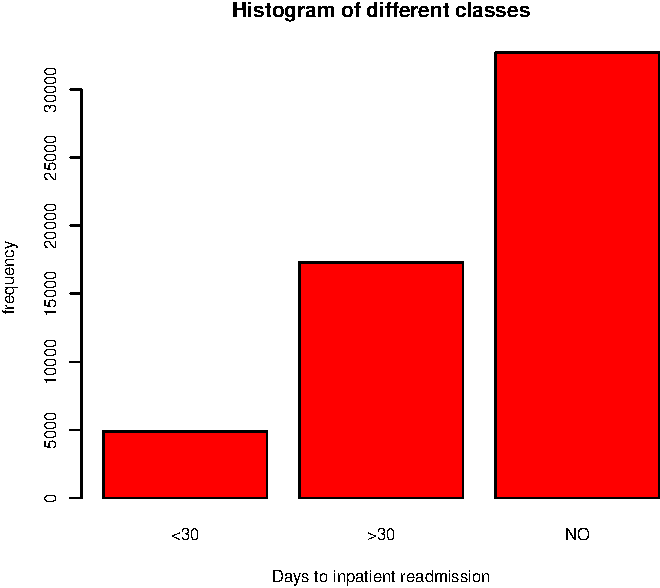
\includegraphics{Project_files/figure-latex/Preprocessing_classtype-1.pdf}

Classes are unbalanced distributed, but not very skewed.

\begin{itemize}
\itemsep1pt\parskip0pt\parsep0pt
\item
  Kill unimportant features.(\emph{nearZeroVar} diagnoses predictors
  that have one unique value (i.e.~are zero variance predictors) or
  predictors that are have both of the following characteristics: they
  have very few unique values relative to the number of samples and the
  ratio of the frequency of the most common value to the frequency of
  the second most common value is large.) (cite)
\end{itemize}

\begin{Shaded}
\begin{Highlighting}[]
\NormalTok{NZV <-}\StringTok{ }\KeywordTok{nearZeroVar}\NormalTok{(training,}\DataTypeTok{saveMetrics =} \NormalTok{T)}
\NormalTok{training <-}\StringTok{ }\NormalTok{training[,-}\KeywordTok{which}\NormalTok{(NZV$nzv==}\OtherTok{TRUE}\NormalTok{)]}
\end{Highlighting}
\end{Shaded}

\begin{itemize}
\itemsep1pt\parskip0pt\parsep0pt
\item
  Kill same features for \texttt{test} dataset without looking inside.
\end{itemize}

\begin{Shaded}
\begin{Highlighting}[]
\NormalTok{test <-}\StringTok{ }\NormalTok{test[,-}\KeywordTok{which}\NormalTok{(NZV$nzv==}\OtherTok{TRUE}\NormalTok{)]}
\end{Highlighting}
\end{Shaded}

\section{Save \texttt{training} and \texttt{test} into csv file for
future use}\label{save-training-and-test-into-csv-file-for-future-use}

\begin{Shaded}
\begin{Highlighting}[]
\NormalTok{if (!}\KeywordTok{file.exists}\NormalTok{(}\StringTok{'training.csv'}\NormalTok{))\{}
    \KeywordTok{write.csv}\NormalTok{(}\KeywordTok{cbind}\NormalTok{(training,training_label),}\StringTok{'training.csv'}\NormalTok{,}\DataTypeTok{row.names =} \OtherTok{FALSE}\NormalTok{)}
    \KeywordTok{write.csv}\NormalTok{(}\KeywordTok{cbind}\NormalTok{(test,test_label),}\StringTok{'test.csv'}\NormalTok{,}\DataTypeTok{row.names =} \OtherTok{FALSE}\NormalTok{)}
\NormalTok{\}}
\end{Highlighting}
\end{Shaded}

Purpose for doing that is \texttt{R} is good for exploratory research,
but not good at dealing with large dataset for clasification. Use
\texttt{Python} to read csv as \texttt{SFrame} for classification will
speed up! (cite)

\end{document}
